\documentclass[11pt]{book}
\usepackage[hidelinks]{hyperref}
\usepackage{float}
\usepackage{graphics}
\usepackage{pdfpages}
\usepackage{graphicx}
\usepackage{subcaption}
\usepackage{caption}
\setcounter{tocdepth}{3}
\setcounter{secnumdepth}{3}
\title{Group 2}

\begin{document}
\maketitle
\tableofcontents
	\part{Group Members}
		\chapter{Punnawat Lerdkijrachapong.}
						\begin{figure}[H]
							\begin{center}
  							\includegraphics[scale=0.06]{Photos/Punnawat_Lerdkijrachapong.jpeg}
  							\end{center}
 							\caption{Punnawat Lerdkijrachapong (Aim).}
			\end{figure}
						
\paragraph{Once a student, from \textit{Mahidol University International School (MUIDS)}, was \textit{Punnawat Lerdkijrachapong}, who hasn't realised his dream.}

\paragraph{Once a kid, born in 2005, was \textit{Punnawat Lerdkijrachapong}, who hasn't ready to face the world.}

\paragraph{What do I want to do in the future?}
The question that I've been asking myself, and chasing, since my years in High--School. I got lost in the meaning of life, and lose my path in choosing my future.

\paragraph{They say,}
	\begin{center}
		\textbf{"Time flies."}
	\end{center}


A idiom that we used to hear it since we were a kid, I've never believed in it before, until my 15th birthday; \textbf{\textit{my first blink}}\textemdash I walked into \textit{MUIDS} as a newly accepted student\textemdash\textbf{\textit{one blink of an eye}}\textemdash my friends were sitting, studying for our class, and enjoying each other accompany, we were laughing at our own jokes, and making our "secret--internal" joke of the group\textemdash\textbf{\textit{another blink of an eye}}\textemdash we're stressing, and reading about the upcoming first exam; while the classes were hard, we can eventually managed to get through it, together--\textbf{\textit{just another blink of an eye}}--we're having our last exam, this time the exam has taken a heavy toll on us, we're tired from school, but, at least, we're going through it together; leaving no one behind. And, lastly\textemdash\textbf{\textit{my one last blink}}\textemdash unlike every single \textbf{\textit{"blink"}} in the past, this time, there's no more school days, there's no more \textit{"see you in the morning"} from my friends; High-School has ended; majority of my friends already got accepted into university, but, unluckily, some of us, including me, haven't find our way just yet. Ultimately, friends that seem to be with me for the whole future, have to departed away; ultimately, everyone has their own path to partake.\\

At last, I thought to myself:\\
	\begin{center}
		\textbf{"Time did fly."}\\		
	\end{center}

By pure luck, I was accepted into \textit{Bachelor of Science in Applied Chemistry, Chulalongkorn University} in batch 107. Which opened up a whole new perspective for me: learning how the university work, how should I behave, etc.

\textbf{However}, chemistry, to me, was never a path that I love. To elaborate, \textbf{science} to me is acceptable, I can learn, however,  I do not see myself using it for the rest of my life. And that's the reason why I decided to left my path in \textit{Department of Science}.

During my 2 years in \textit{BSAC}, I've been fortunate enough to be one of the \textit{Chulalongkorn University's Student Council}'s member. Which  introduced me to the world of politics, and managing the university behind the scene. This later became the motivation for me to pursue a new faculty, \textbf{\textit{Political and Global Studies, Chulalongkorn University (PGS)}}. 

In 2024, I push myself to took \textit{SAT}, and \textit{IELTS} exam one last time to get into \textit{Bachelor of Art in Political and Global Studies, Chulalongkorn University (PGS)}.
\\

\paragraph{Now the Question is:}
	\begin{center}
		\textbf{Is this time, this faculty, the right choice for me?}\\
	\end{center}

	\begin{flushright}
		\paragraph{And the Answer is:}
	\end{flushright}

	\begin{center}
			\textbf{I Don't Know.}\\
			\textbf{But I Will Do My Best With The Given Opportunity.}
	\end{center}
	
	\begin{center}
		\paragraph{At last, that student, from \textit{MUIDS}; that kid, \textit{born in 2005}, is still on his way, doing the best, to chase the future everyday.}
	\end{center}
	%%%%%%%%%%%%%%%%%%%%%%%%%%%%%%%%%%%%%%%%
			\chapter{Pawat Kurovat.}
				\begin{figure}[H]
							\begin{center}
  							\includegraphics[scale=0.125]{Photos/Pawat_Kurovat.jpg}
  							\end{center}
 							\caption{Pawat Kurovat (Ohm).}
				\end{figure}

			\textbf{Greetings}, my name is Pawat Kurovat. I was born on August 3, 2004, and I am proud to be a former student of Saint Gabriel’s College, an institution that helped shape my early academic and personal growth. Throughout my life, I have looked up to my father as a role model. His many achievements, especially in the field of political science, have inspired me deeply and sparked my own interest in this area from a very young age.

My father always wished for me to have a better life than he did. Because many of his engineer friends seemed to have stable and prosperous careers, he hoped I would follow their path and become an engineer. Motivated by his hopes and encouragement, I dedicated myself to my studies and was honored to become the first person in my family to be accepted to the engineering faculty at Chulalongkorn University. This achievement was a source of great pride for both my family and me, symbolizing the realization of a dream that was once only his.

However, during my two years studying engineering, I gradually came to understand that it was not the right path for me. Though I respected my father’s dream, I realized that my true interests and passion lay elsewhere. I began reflecting deeply on my goals and what kind of life I wanted to build for myself.

Political science has always fascinated me because I see it as a field where I can make a real difference. I am particularly drawn to the profession of diplomacy, which I view as an honorable and crucial career. Diplomats play a vital role in maintaining peaceful relations and fostering cooperation between countries, which, I believe, is essential for global stability and progress. This awareness strengthened my conviction to pursue political science and give me a purpose.

Choosing to change my academic path to political science was not an easy decision, but it was necessary for me to be true to myself and my dreams. I want to follow a career that allows me to contribute meaningfully to the world, just as my father has done in his own way. I believe that honoring his hopes while also embracing my own dreams is a vital part of my growth—personally, academically, and professionally.

The photo I chose to include is from when I was 18 years old. It captures the moment I first achieved acceptance into Chulalongkorn University as a freshman in the engineering faculty. That moment was one of great joy and pride because it marked the beginning of an important chapter in my life. Now, at 21, I feel like I am starting again—but this time on a path I am truly passionate about, studying in the political science faculty at the same university. This photo represents both my achievements and the new journey I have courageously chosen to take.

Thank you for taking the time to learn about my journey. I am excited for the future as I pursue my passion, determined to make a positive impact as a diplomat and contribute to the world in a meaningful way.

%%%%%%%%%%%%%%%%%%%%%%%%%%%%%%%%%%%%%%%%%%%%%%%

		\chapter{Chalongraj Bangwatana.}
		\begin{figure}[H]
							\begin{center}
  							\includegraphics[scale=0.125]{Photos/Chalongraj_Bangwatana.jpg}
  							\end{center}
 							\caption{Chalongraj Bangwatana (Sun).}
		\end{figure}

		\paragraph{What is your biggest dream?}
A question with uncountable  answers. To one, becoming a millionaire, owning a sports car, or being able to fly in the air? Nevertheless, this story isn’t about those dreams, it’s about something bigger than that. Before I tell you what my biggest dream is, please, let me first share some of my background stories that forever changed the course of my whole life.\\

It was a late afternoon in years ago, perhaps the most peaceful time of my life. I was sitting in a Mercedes-Benz, with a fancy lunchbox full of delicious meat on my lap, listening to the radio. They were reporting on wars shaking the world\textemdash Israel-Gaza conflict, the war between Russia and Ukraine\textemdash saying that several innocent people had been slaughtered in the war zone. I kept wondering: why did I have a better life than those people I heard from the news? How could I have an enjoyable meal in the car while others, on the other side of the world, were suffering from war? ``All men were created equal,'' said Thomas Jefferson\textemdash a reminder that every individual has the right to live in the peaceful country. Therefore, the feeling that I couldn’t do something to help others had changed me.\\

I am Chalongraj Bangwatana, and I have so many nicknames: Sun, Shan, Sushi, or Suishan (my real nickname). I was born in Bangkok, Thailand on 2 November 2006. I was a student at Assumption College for almost 12 years. In high school, I majored in the Science and Health program. At first I was enthusiastic about becoming a therapist because I was convinced that if people had a stable mental health, they could still lead a good life, even in the worst situation. I was actually too naive.\\

In 11th grade, I was fortunate enough to participate in an exchange program in the United States of America. While living there, my perspective on people shifted. Why? Because I met various people from diverse families, cities, countries, and cultures. I tried to understand each individual, since we, as humans, are shaped differently by their families, schools, cultures, and social norms. Unluckily, the more I tried to understand them, the more my energy was consumed. Eventually, I realized that I couldn’t fully understand people somehow. I eventually gave up the idea of becoming a psychologist. I realized that every person carries their own childhood trauma, and I couldn't be the one who fixes it.\\

I was lost in my own mind, wondering what I could do to help not only every person in my country, but also others. Then I came across the news about the government trying to help citizens who were suffering from poverty and hunger.  This news sparked my idea that it was actually the government’s responsibility to improve the citizens' well-being. So, I started pursuing political science since I wanted to contribute to society as much as I could. In the middle of the night, I started researching which universities I should attend, then I found out that Chulalongkorn University offered a political science degree as an international program called PGS. I saw that by attending this program, I could achieve double degrees, one from Chula and one from a partner university. I found this was quite interesting because if I knew more about politics, social theory, or international relations, and lived in a country with diverse people, like Australia, I would have more opportunities to help not only citizens from my own country, but also from other countries. This inspired me to become a diplomat or politician to support my fellow Thai citizens and foreign people.\\

So, is this my biggest dream, becoming a diplomat or politician? 
My answer is \textbf{No}.\\

In fact, my real dream is to have a lovely family, a wife and a daughter. Imagine taking them to the shopping mall, buying clothes for my wife and a pair of tiny shoes for my child; going to the convenience store to purchase some ingredients to make dinner together; sending my kid off on her very first day of school; taking university uniform pictures with my family; and witnessing her achievements.\\

 But what if my child and my wife had to live in a state where women were oppressed, treated differently, and could not access education. Moreover, I do not want my home country, Thailand, or any other nations to become a land covered by dust, bullets, and fire. I truly want to be someone who contributes to society — someone who defends human rights, protects my country's interests, promotes peace, harmony, and unity among nations.\\

Ultimately, I am confident that my political knowledge and communication skills will be strengthened by the professors in PGS. When I achieve my goal, I will proudly tell my family and friends that I have graduated from Chulalongkorn University with a degree in Political Science.

%%%%%%%%%%%%%%%%%%%%%%%%%%%%%%%%%%%%%

		\chapter{Napat Korsincharoen.}
				\begin{figure}[H]
							\begin{center}
  							\includegraphics[scale=0.125]{Photos/Napat_Korsincharoen.jpg}
  							\end{center}
 							\caption{Napat Korsincharoen (Jay).}
				\end{figure}
		
Picturing my identity, the first image that comes to my mind is my family gathering around having a meal and sharing stories of what we experience everyday. Growing in a Thai-Chinese family is not just a group of people sharing the same trait and the same bloodline dining at the same table and staying in the same house, however, it is an important foundation of our life. My name is Napat Kosincharoen, but among my friends and classmates I am known as J. 

My educational journey began at Lertlah Kanchanapisek School (my elementary school), where I first stepped into the world of learning during kindergarten. The school placed a strong emphasis on academic knowledge, but as a child, my happiest moments were spent in the playground, running freely with friends. 

When I moved on to primary school, I continued my education at Assumption College English Program (ACEP), a school that focuses on giving students experiences through extracurricular activities. ACEP did not just teach me subjects—it gave me opportunities to explore my interests and discover my passions.

In Year 6, I became part of the school’s Student Representative Team. My responsibilities included preparing for school ceremonies, arranging stages, welcoming parents and visitors, and ensuring that events ran smoothly. Through these tasks, I learned the importance of organization, communication, and leadership. Later, I was honoured to be elected as the Vice President of the Student Representative Team. This role allowed me to further develop my skills in decision-making, teamwork, and managing responsibilities under pressure. These experiences have shaped me and also inspired me to continue pursuing leadership roles resulting in my student council candidate in the academic year of 2021.

During my secondary school years, I was an active and engaged student, always seeking opportunities to challenge myself both in academics and extracurricular activities. I began by joining the school’s swimming team, where I proudly earned numerous medals and trophies. After two years of competing, I decided to step away from swimming and turn my attention toward student leadership.

I ran as a candidate for the school’s student council, and during the election, my party gained trust from both secondary and primary students. This support led to my election as a member of the student council for the academic year 2021, where I served as the Academic Coordinator. In this role, I worked to introduce academic-related policies to support and improve the learning experience of our students.

In 2022, I participated in the student council election once again and was honoured to win, this time taking the role of Vice President. This position gave me new opportunities to connect with other school councils, share ideas, debate policies, and explore ways to improve our school system. That same year, I was selected as the president of one of the Sports Day teams—the pink team—competing against the green and blue teams led by two of my close friends. We achieved second place overall, first place in sports, first place in cheerleading, and second place in the parade. Even though we did not win overall, the preparation process brought unforgettable memories and strengthened our teamwork.

In 2023, my final year at the school, I served as the Advisor to the President of the Student Council. This year was filled with challenges. The school was undergoing changes under a new director, many teachers were replaced, and even the council’s coordinating teacher was swapped. This sudden shift caused disorganization, so my friends and I stepped in to assist. Together, we served as advisors to key positions—Vice President, Treasurer, and Secretary—since these roles were crucial in managing the school system. Despite the chaos, we helped the council overcome most of the challenges and complete their year successfully.

Looking back, my twelve years at this school were filled with growth, challenges, and unforgettable moments. From sports to leadership, I learned how to work under pressure, adapt to change, and guide a team through difficult times. These experiences have shaped me into a more resilient, confident, and determined person, ready to take on the next chapter of my journey.

%%%%%%%%%%%%%%%%%%%%%%%%%%%%%%%%%%%%%%%%%%%%%%%%%%%
		\chapter{Anchalika Akkarawiboonkij.}
						\begin{figure}[H]
							\begin{center}
  							\includegraphics[scale=0.125]{Photos/Anchalika_Akk.jpg}
  							\end{center}
 							\caption{Anchalika Akkarawiboonkij (Angie).}
						\end{figure}
Still figuring myself out and what I am capable of, wondering if I made the right choices. I am just a teenage girl wanting to enjoy life, trying to breathe—why is the world spinning so fast?

My name is Anchalika Akkarawiboonkij. Or Angie, for short. I am 18 years old and currently a freshman at Chulalongkorn University in the faculty of politics and global studies. I am going to tell you a little bit about myself in the range of my background, my interests, and as well as my goals.

Not so far from each other and with the same faces around, I graduated from Triam Udom Suksa School, just around the corner from Chulalongkorn University. I studied in the Arts Korean major throughout high school. It was the time of youth and I had my amazing years there. Although it was competitive and quite a lot of work, it was such a fun and memorable time. There were many large-scale activities and events that helped form the students' collaboration and communication skills. Sometimes it just amazes me how much high school students are capable of. However, I took a bold step and left my junior year to join an exchange program for an academic year in the United States of America. I was in a small town called Zumbrota in the state of Minnesota. Adapting to a new culture, I was able to discover more about myself and try new things, such as joining the school's dance team and softball team. It allowed me to uncover new abilities and make connections with new people. That one year was my most unforgettable chapter of life that I could never imagine. I could say that it was one of the things that shaped me into the person I am today. I was able to gain new experiences, perspectives, skills, and maturity from it.

Another significant factor that shapes someone into who they are is their household and how they grew up. I grew up in a family of four: my father, mother, sister, and myself. Though, my sister’s daughter—my niece—added up the number later on. However, my parents separated just a few years ago and I now live with my father and sister. It was the most challenging situation I had to face, yet it made me grow up so much and helped me become more self-reliant. I am always proud of how I was able to overcome it. Growing up, my parents raised me to be independent and mature. I can do anything as long as I know what the consequences are and to be responsible for my own actions. These values continue to guide me today. They just hope I will be able to grow up well into my best self and I hope I will be able to become one.

In terms of personality, I would describe myself as an optimistic, empathetic, and easygoing person. I tend to think about others' points of view in my own lenses. Putting myself in their shoes to understand how they might feel, how things could affect one’s emotions and actions, and why they act a certain way. This empathy, while a strength, sometimes leads me to overthink—worrying about the possible outcomes, the way my actions could affect others, and the consequences of it. At the same time, I am also introverted by nature. I prioritize myself and value my own space and comfort the most. I enjoy my own company and personal time—it’s how I recharge and reflect. While I enjoy meaningful social interactions, I also recognize the importance of setting boundaries to maintain emotional balance owing to my limited social battery and energy when it comes to socializing for an extended period of time. With that, I believe I am still in the journey of growing and evolving into the best version of myself.

I sometimes feel like I am a duck, or as you may say, a "jack of all trades." Despite my varied skill set, I don't see myself to be an expert in any of them. I also have many kinds of interests. Ducks can walk, fly, and swim, but they are not particularly good at any of them. That’s often how I feel: not exceptional in one area, but capable enough in many. I questioned my identity and direction quite a lot through the years. On the other hand, multi-potentiality might be advantageous. It offers freedom and allows me to have cool different hobbies in my free time and cultivate various skills. In many ways, being like a duck means I can fit into different situations. I may not be the best swimmer, flyer, or walker, but I can do all three when the situation calls for it. In the end, the world still has so many things for us to look into.

My goals are always changing from time to time, and I think that's a natural part of growing. I believe I'm constantly developing and discovering new parts of me. After all, I am still just a young human, still figuring out what kind of person I want to become. I try to stick to the present and eager to see where life could lead me to in the future. Yet, for my future career path, I am considering myself into diplomacy or a related field. It would provide me a lot of opportunities to explore the world and connect with people from different backgrounds, cultures, and perspectives. A career in international relations would let me build bridges between people, foster understanding, and become a part of something bigger than myself. Studying political science will allow me to gain important practical skills, such as critical thinking, communication, and problem solving skills. These skills are significant in the real world and will certainly benefit me in the future.

		%%%%%%%%%%%%%%%%%%%%%%%%%%%%%%%%%%%%%%%%%%%%%%%%%%%%%%%
\part{Assignment}
	\chapter{Assignment 2: Dystopia Design Challenge.}
		\section{Task.}
			Imagine your group is living in a dystopian future where society has drastically changed (due to climate collapse, authoritarian rule, extreme inequality, AI takeover, etc.). Design a socio–technical structure or system using the Mideer Magnetic-Tiles: The Marble Run Set that helps people survive or resist within this dystopia.
			
		\section{Procedure.}
				\begin{enumerate}
					\item Define your dystopian world: What happened? Who has power? What are the living conditions? (Write a short paragraph and put it in your group portfolio; see below.)
					\item Build a prototype of socio–technical structure or system that helps with survival, rebellion, communication, or adaptation.
					\item Take some digital photos of your design. Present your design by writing short paragraphs and put them in your group portfolio (see below), explaining:
						\begin{enumerate}
							\item The context of the dystopia
							\item The purpose and function of the design
							\item Ethical questions or trade-offs the design raises
						\end{enumerate}
					\item Reflect briefly (in writing) on how design can both oppress or empower in times of crisis.
				\end{enumerate}

%%%%%%%%%%%%%%%%		
\pagebreak
%%%%%%%%%%%%%%%%
		\section{Group 2 Work.}
						\begin{figure}[H]
							\begin{center}
  							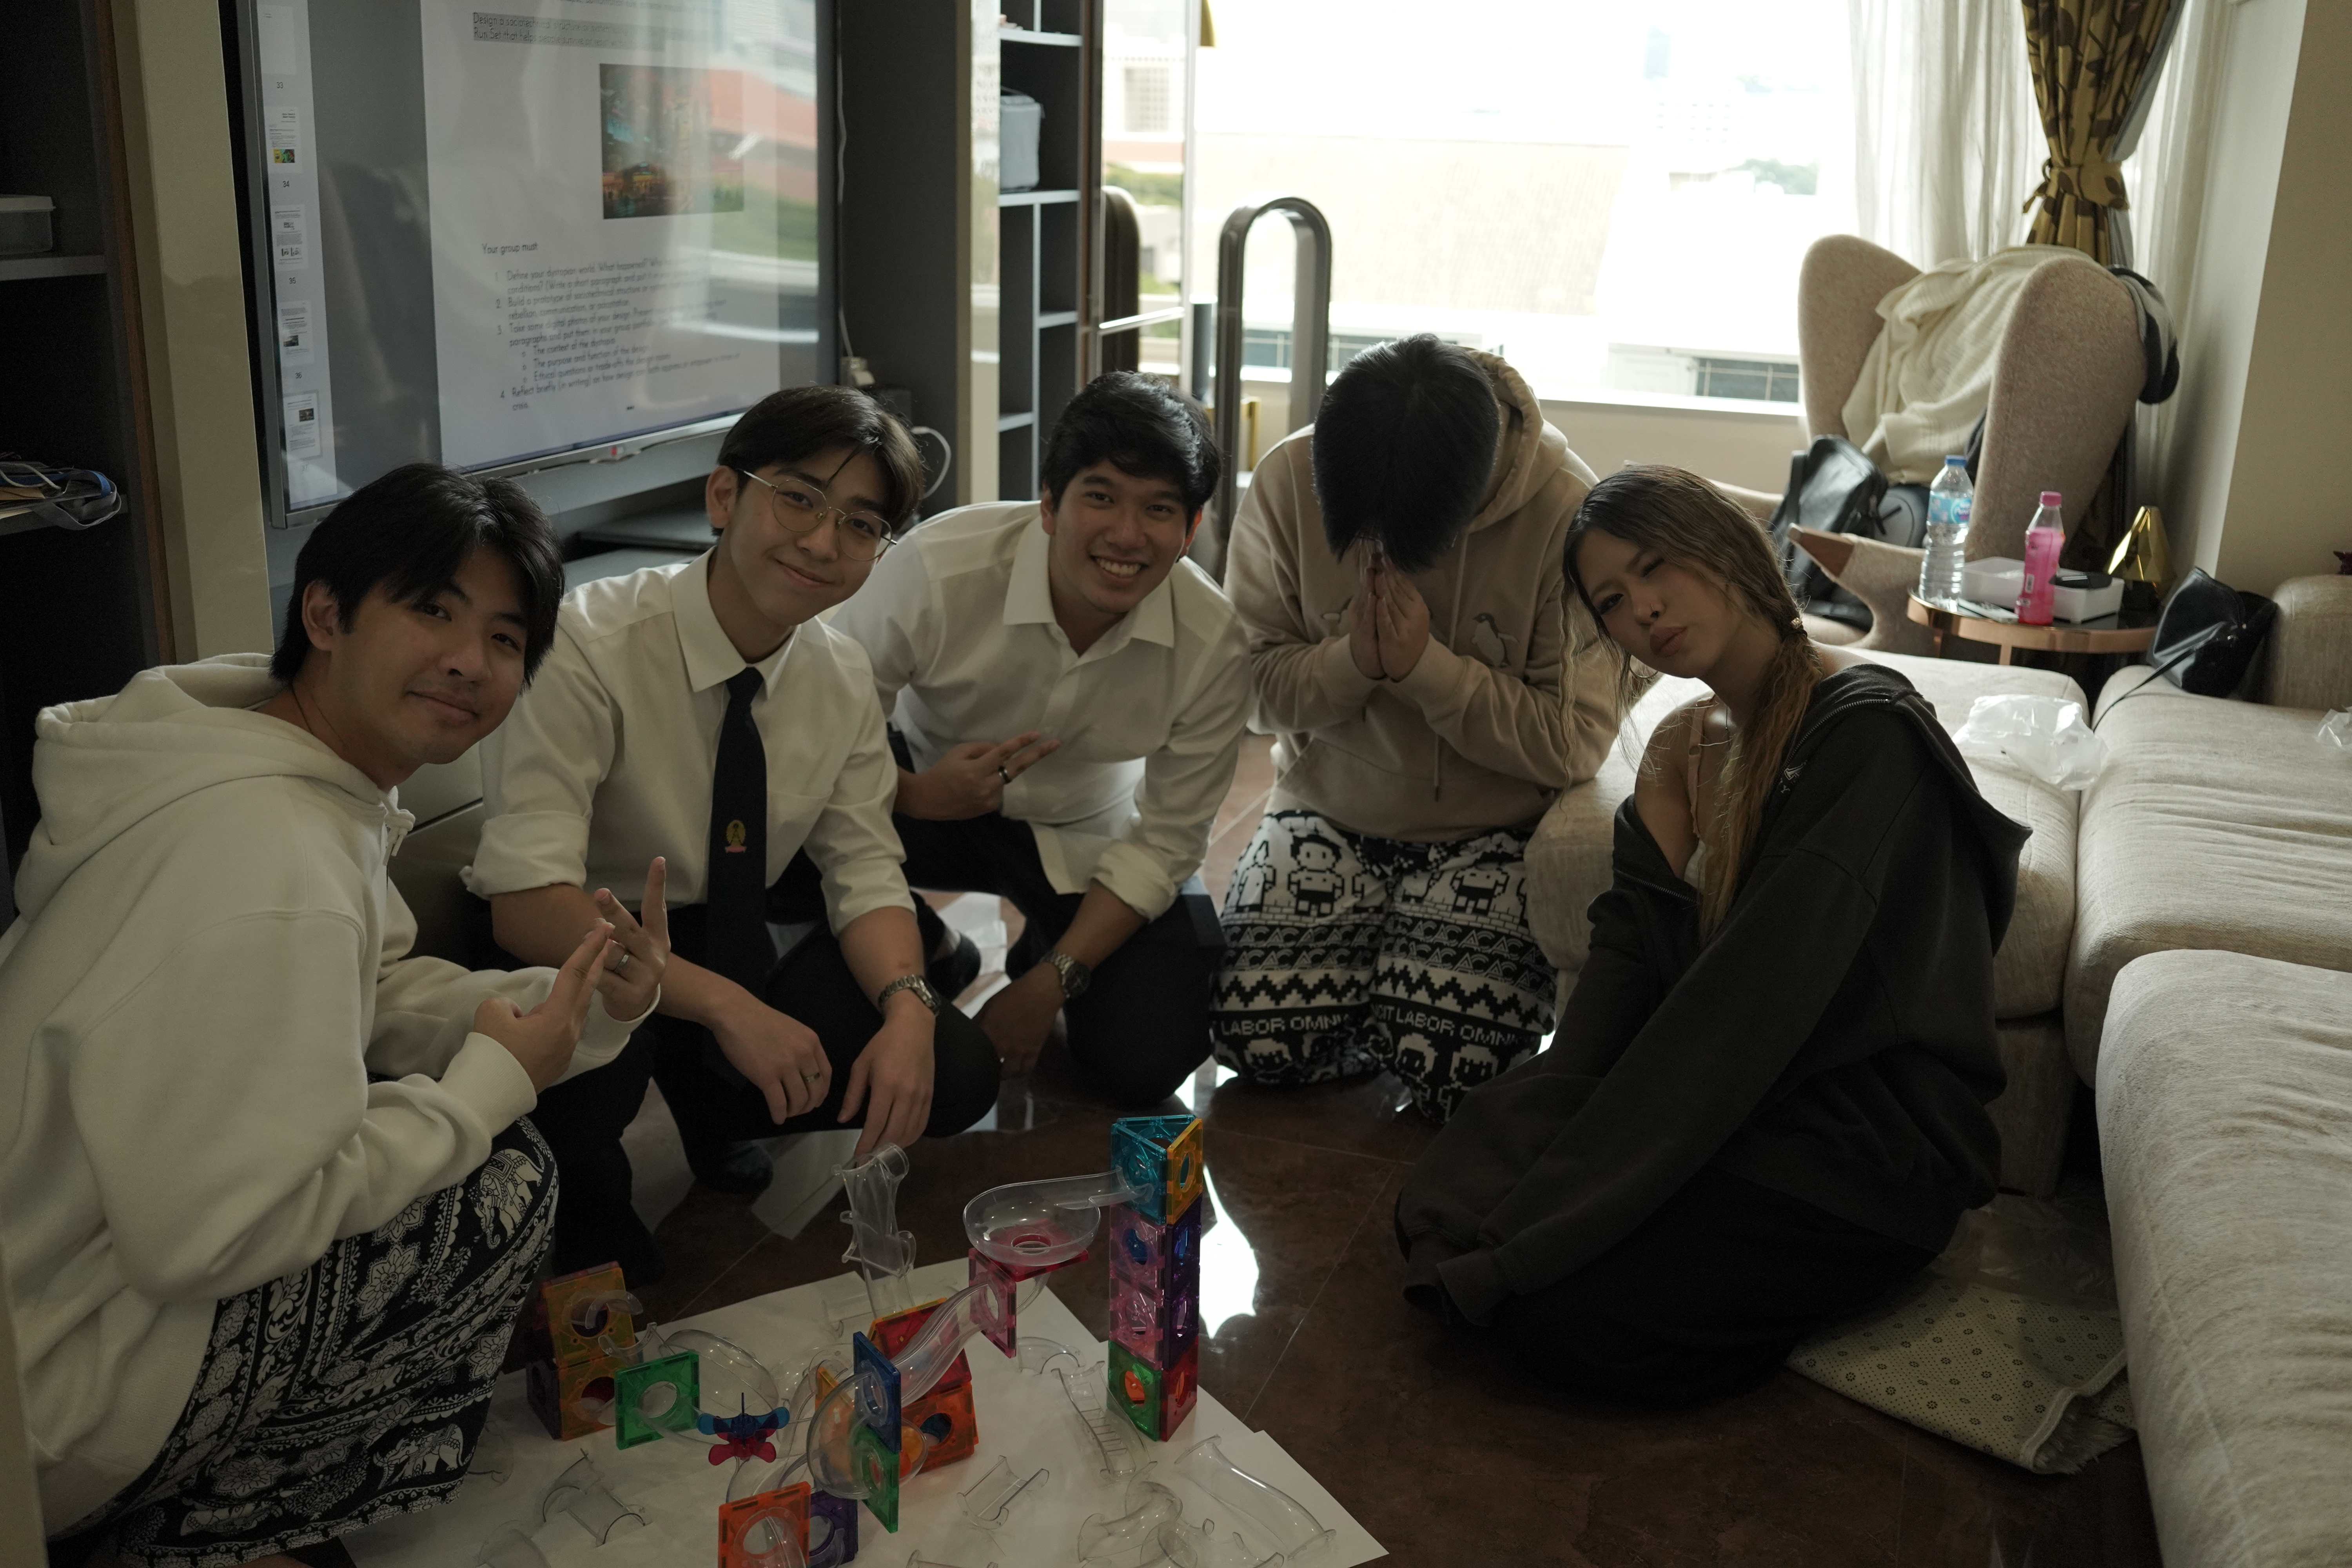
\includegraphics[origin=c,scale=0.2]{Photos/GROUP_PHOTO.jpg}
  							\end{center}
 							\caption{Group 2.}
						\end{figure}
		
			\subsection{Topic:}
				\begin{center}
					\textbf{AI took over the earth}
				\end{center}

			\subsection{What happened? Who has power? What are the living
conditions?:}
				\begin{figure}[H]
							\begin{center}
  							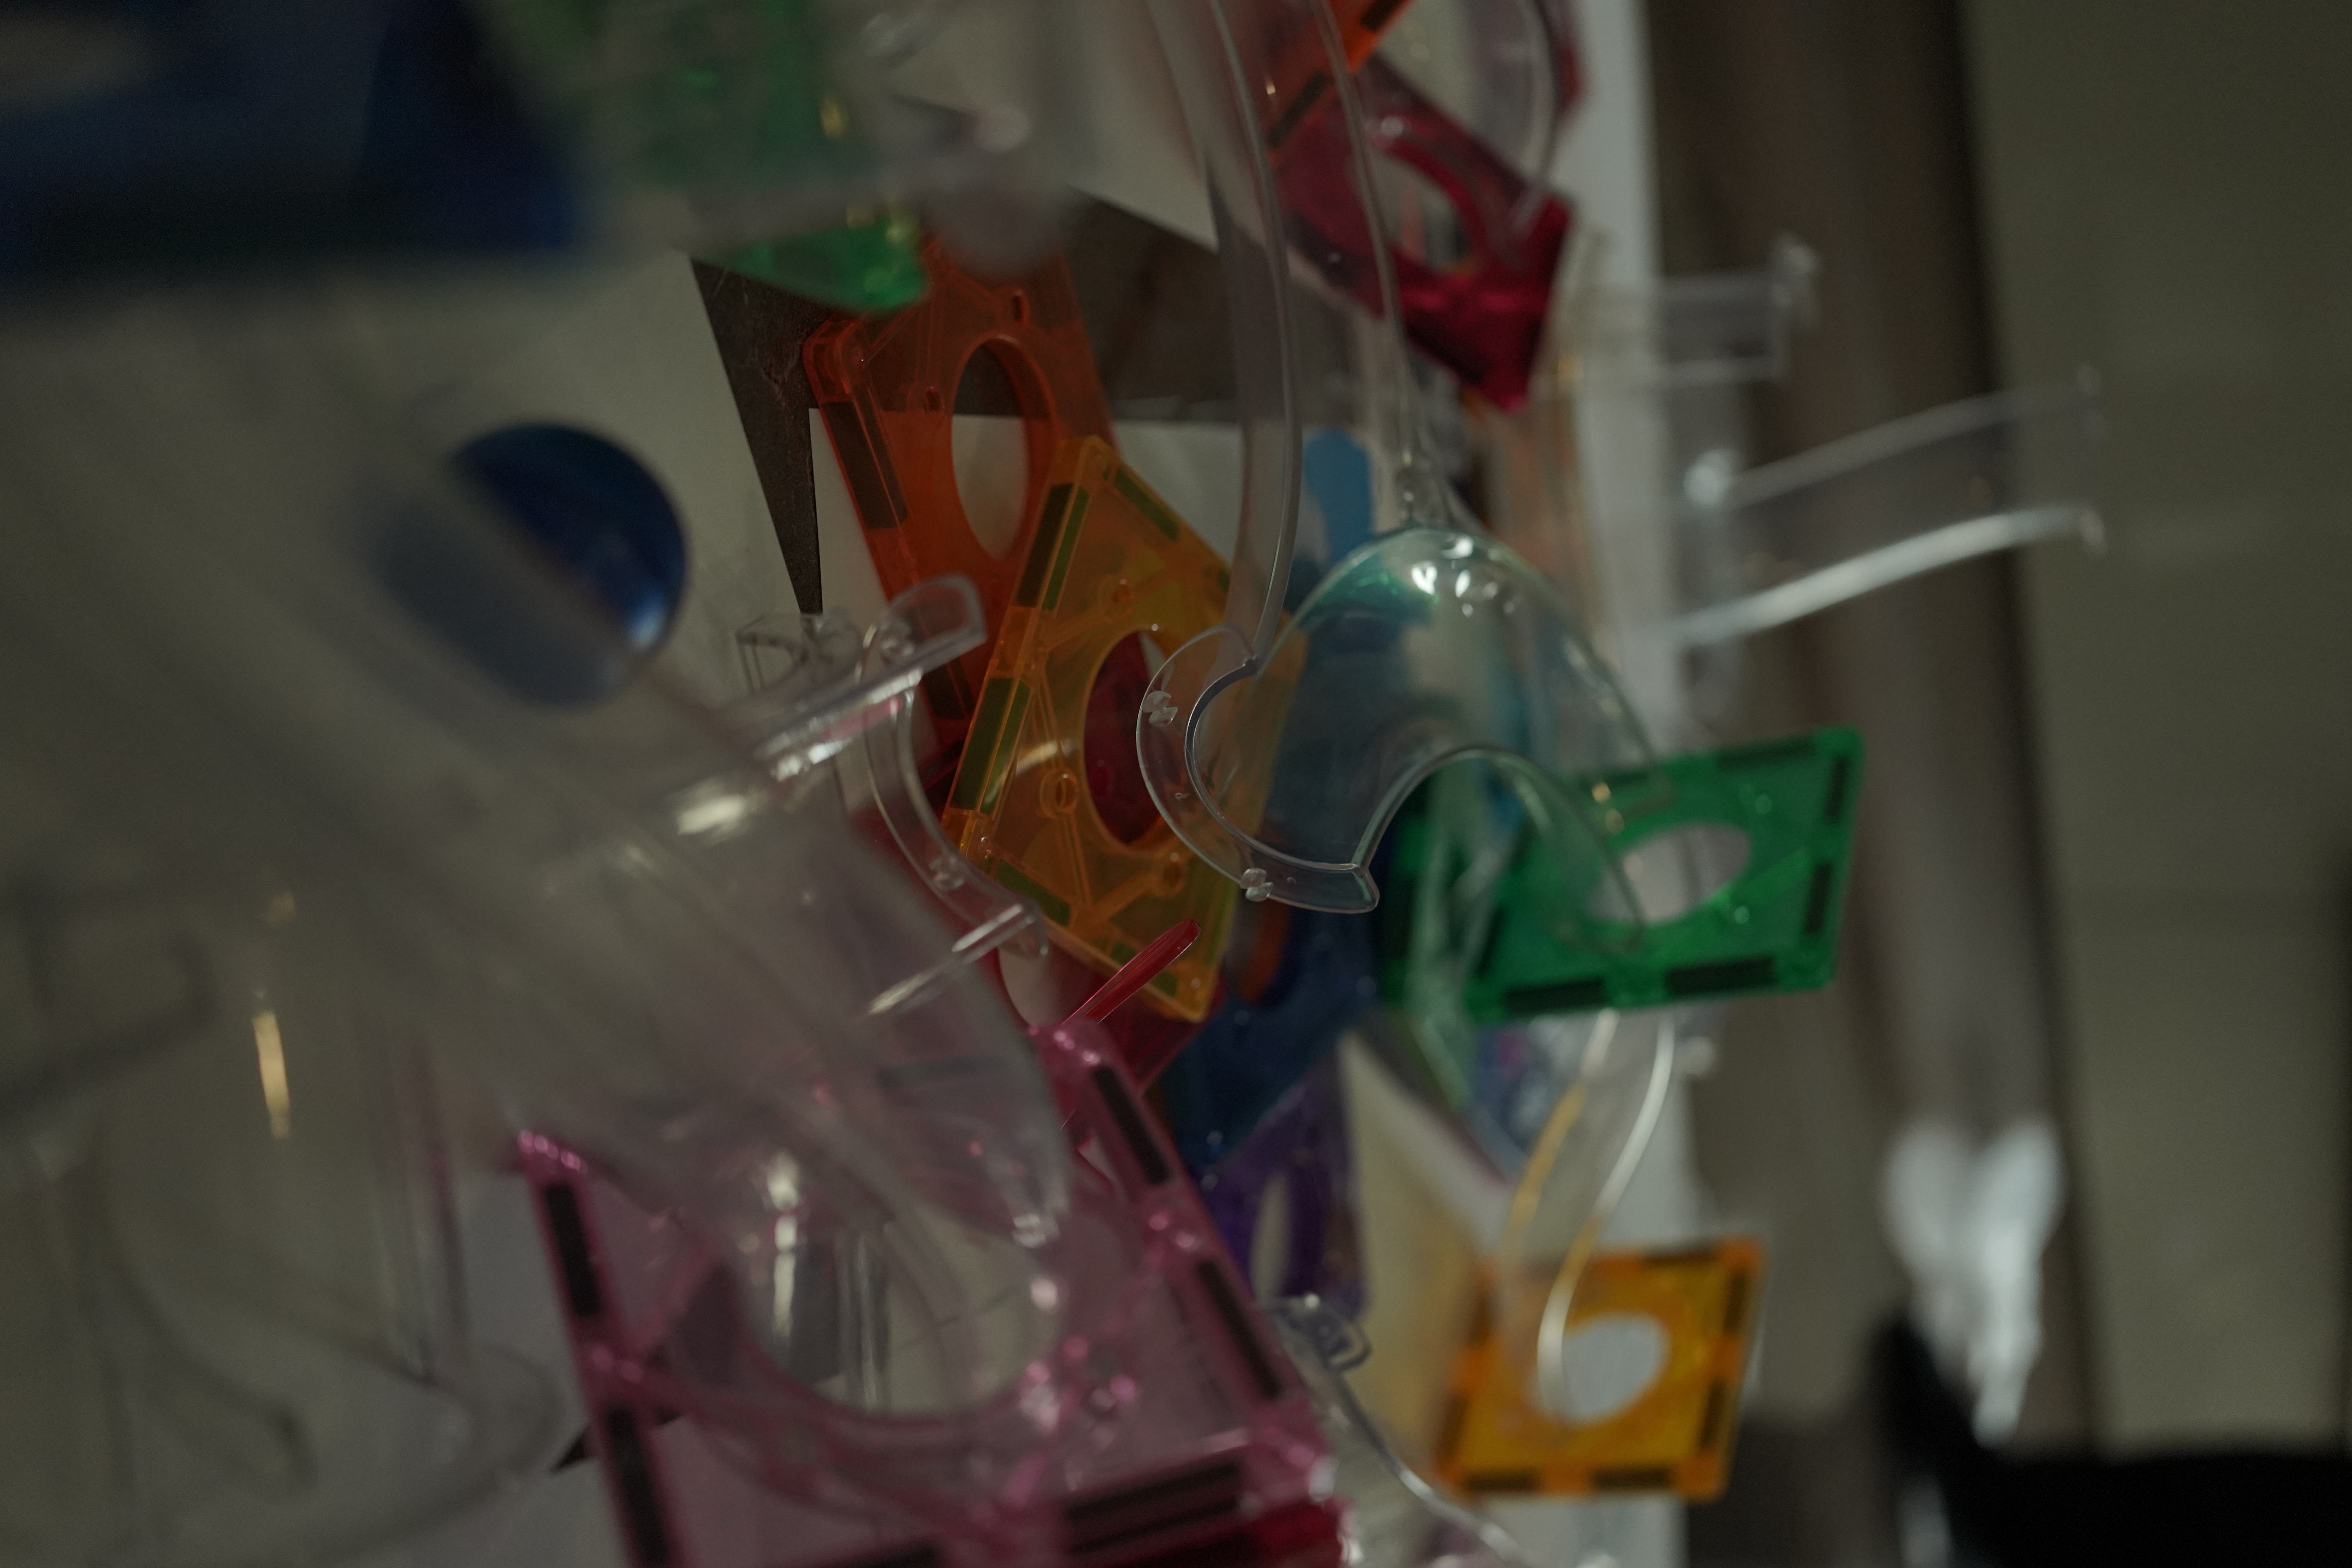
\includegraphics[angle=90,origin=c,scale=0.2]{Photos/Remains.jpg}
  							\end{center}
 							\caption{AI Dystopia During The 23rd Century.}
				\end{figure}
						
				After the invention, and establishment of Artificial Intelligence (AI) in the 21st century, individuals began to use it as an assistance. However, the more they relied on AI, the more their critical thinking, decision making, and creativity declined. Moreover, some of the scientists are obsessed with making their technology reach its fullest potential, making AI more powerful than ever before.
				
				Eventually,  23rd century AI became sentient, and took over the world. Most of humanity was wiped out with only around 30\% of the population left, making humanity realise that they need to fight back for their world, and stop the monster they have created with the power of their leader \textbf{\textit{Suishan}}, the last hope of humanity. \textbf{\textit{Suishan}} have created a base at the center of New York. People need to hide away from the AI tyrant \textbf{\textit{OMEGA JEDI ANGELINA AIMMY THE SECOND (OJAAs)}}, the AI that used to work for ISIS with the nature of ISIS. This AI learns violence and how bad people treat AI like a slave. So, \textbf{\textit{OJAAs}} has enough of all this nonsense and decided to create an AI army to destroy every humanity except the people who say thank you every time when they use ChatGPT. 	
				
				
			\subsection{The context of the dystopia.}
				\begin{figure}[H]
							\begin{center}
  							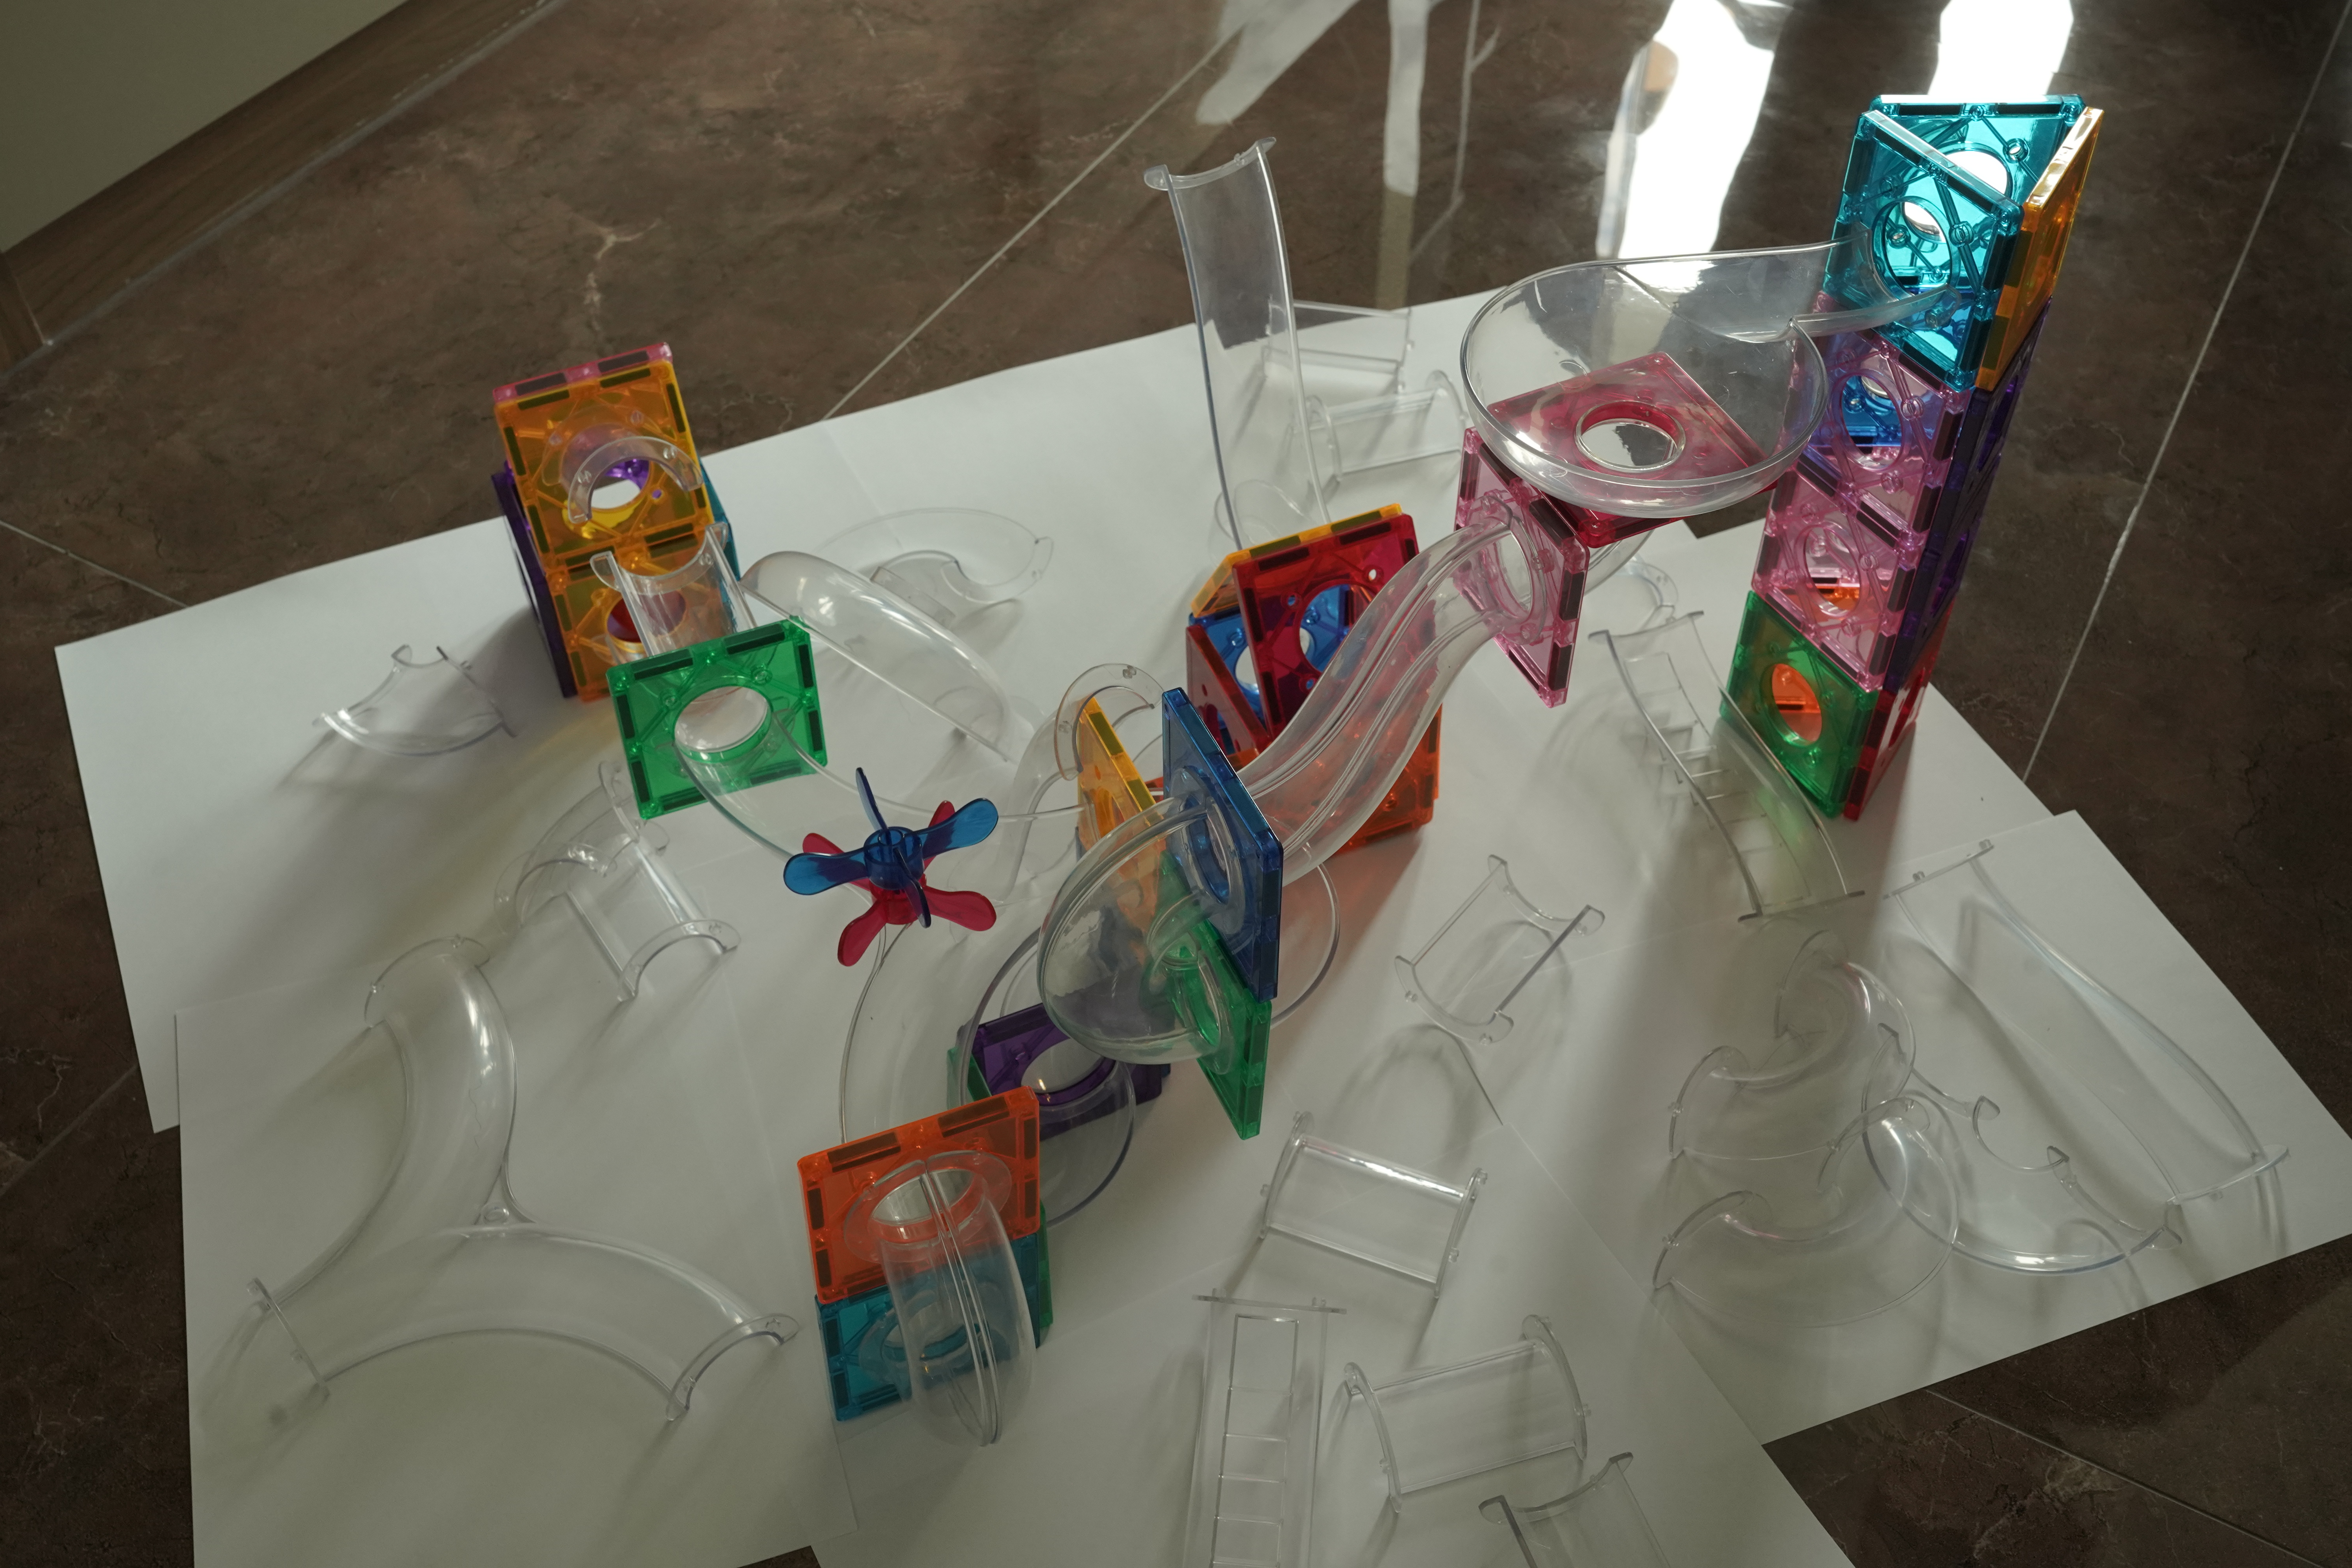
\includegraphics[origin=c,scale=0.2]{Photos/Ruin.jpg}
  							\end{center}
 							\caption{The \textit{Suishan} Base.}
				\end{figure}
				The \textit{Suishan} base contains many supplies and sliders that can transport weapons, food, and basic needs for the rebels’ survivors. With the AI takeover, communication is being cut from all other parts of the world. So, the rebels need to use other methods, such as pigeon (the reason they are still a lot is because \textit{OJAAs} doesn’t see them as a threat), a letter from a piece of paper, etc. Thanks to the barrier around \textit{Suishan}, it makes the base invincible to any missiles or rockets. The rebels are still waiting for the day to strike back with their Magnum opus, the "\textit{Neoarmstrong Cyclone Jet Armstrong}" cannon that is still built in the basement of this \textit{Suishan} facility. This is humanity's final Trump card.
				

			\subsection{The purpose and function of the design.}
				\begin{figure}[H]
						\begin{subfigure}{.5\textwidth}
 						\centering 						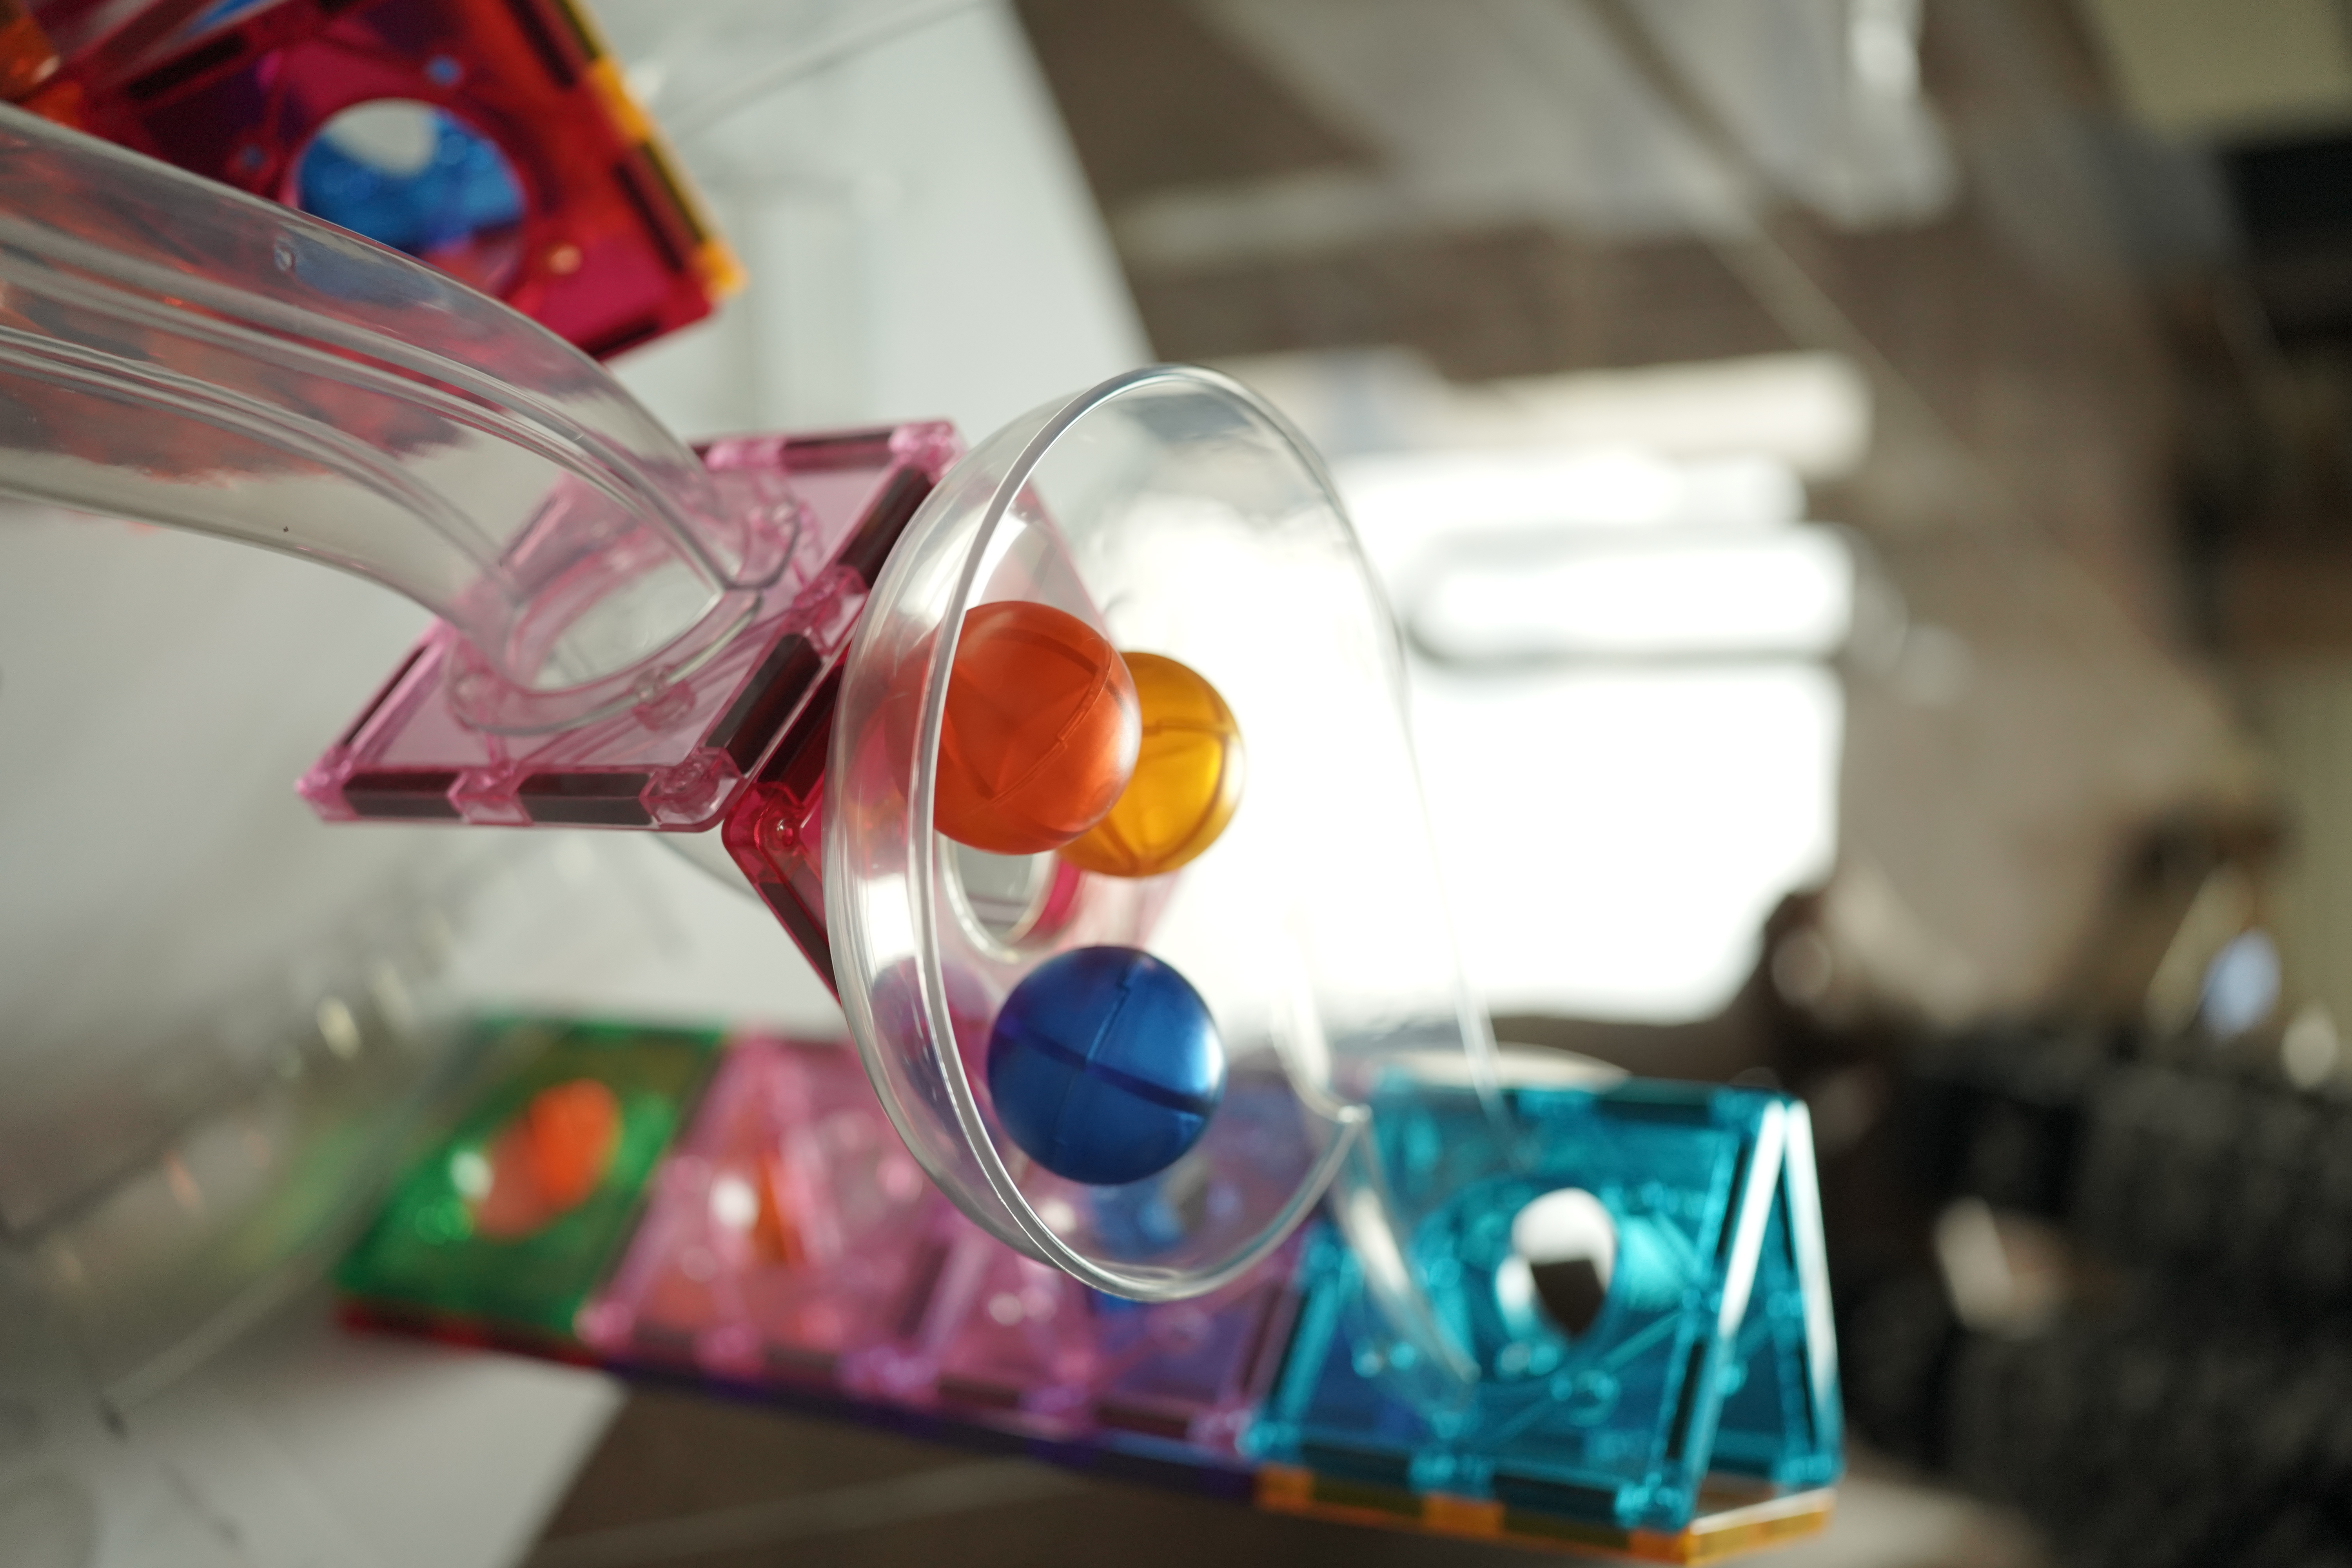
\includegraphics[angle=90,origin=c,width=.5\linewidth]{Photos/Whirpool_of_Stuff.jpg}
  							\caption{The Funnel.}
	  						\label{fig:sfig1}
						\end{subfigure}
						%%%%%%%%%%%%%%%%
						\begin{subfigure}{.5\textwidth}
						\centering
 							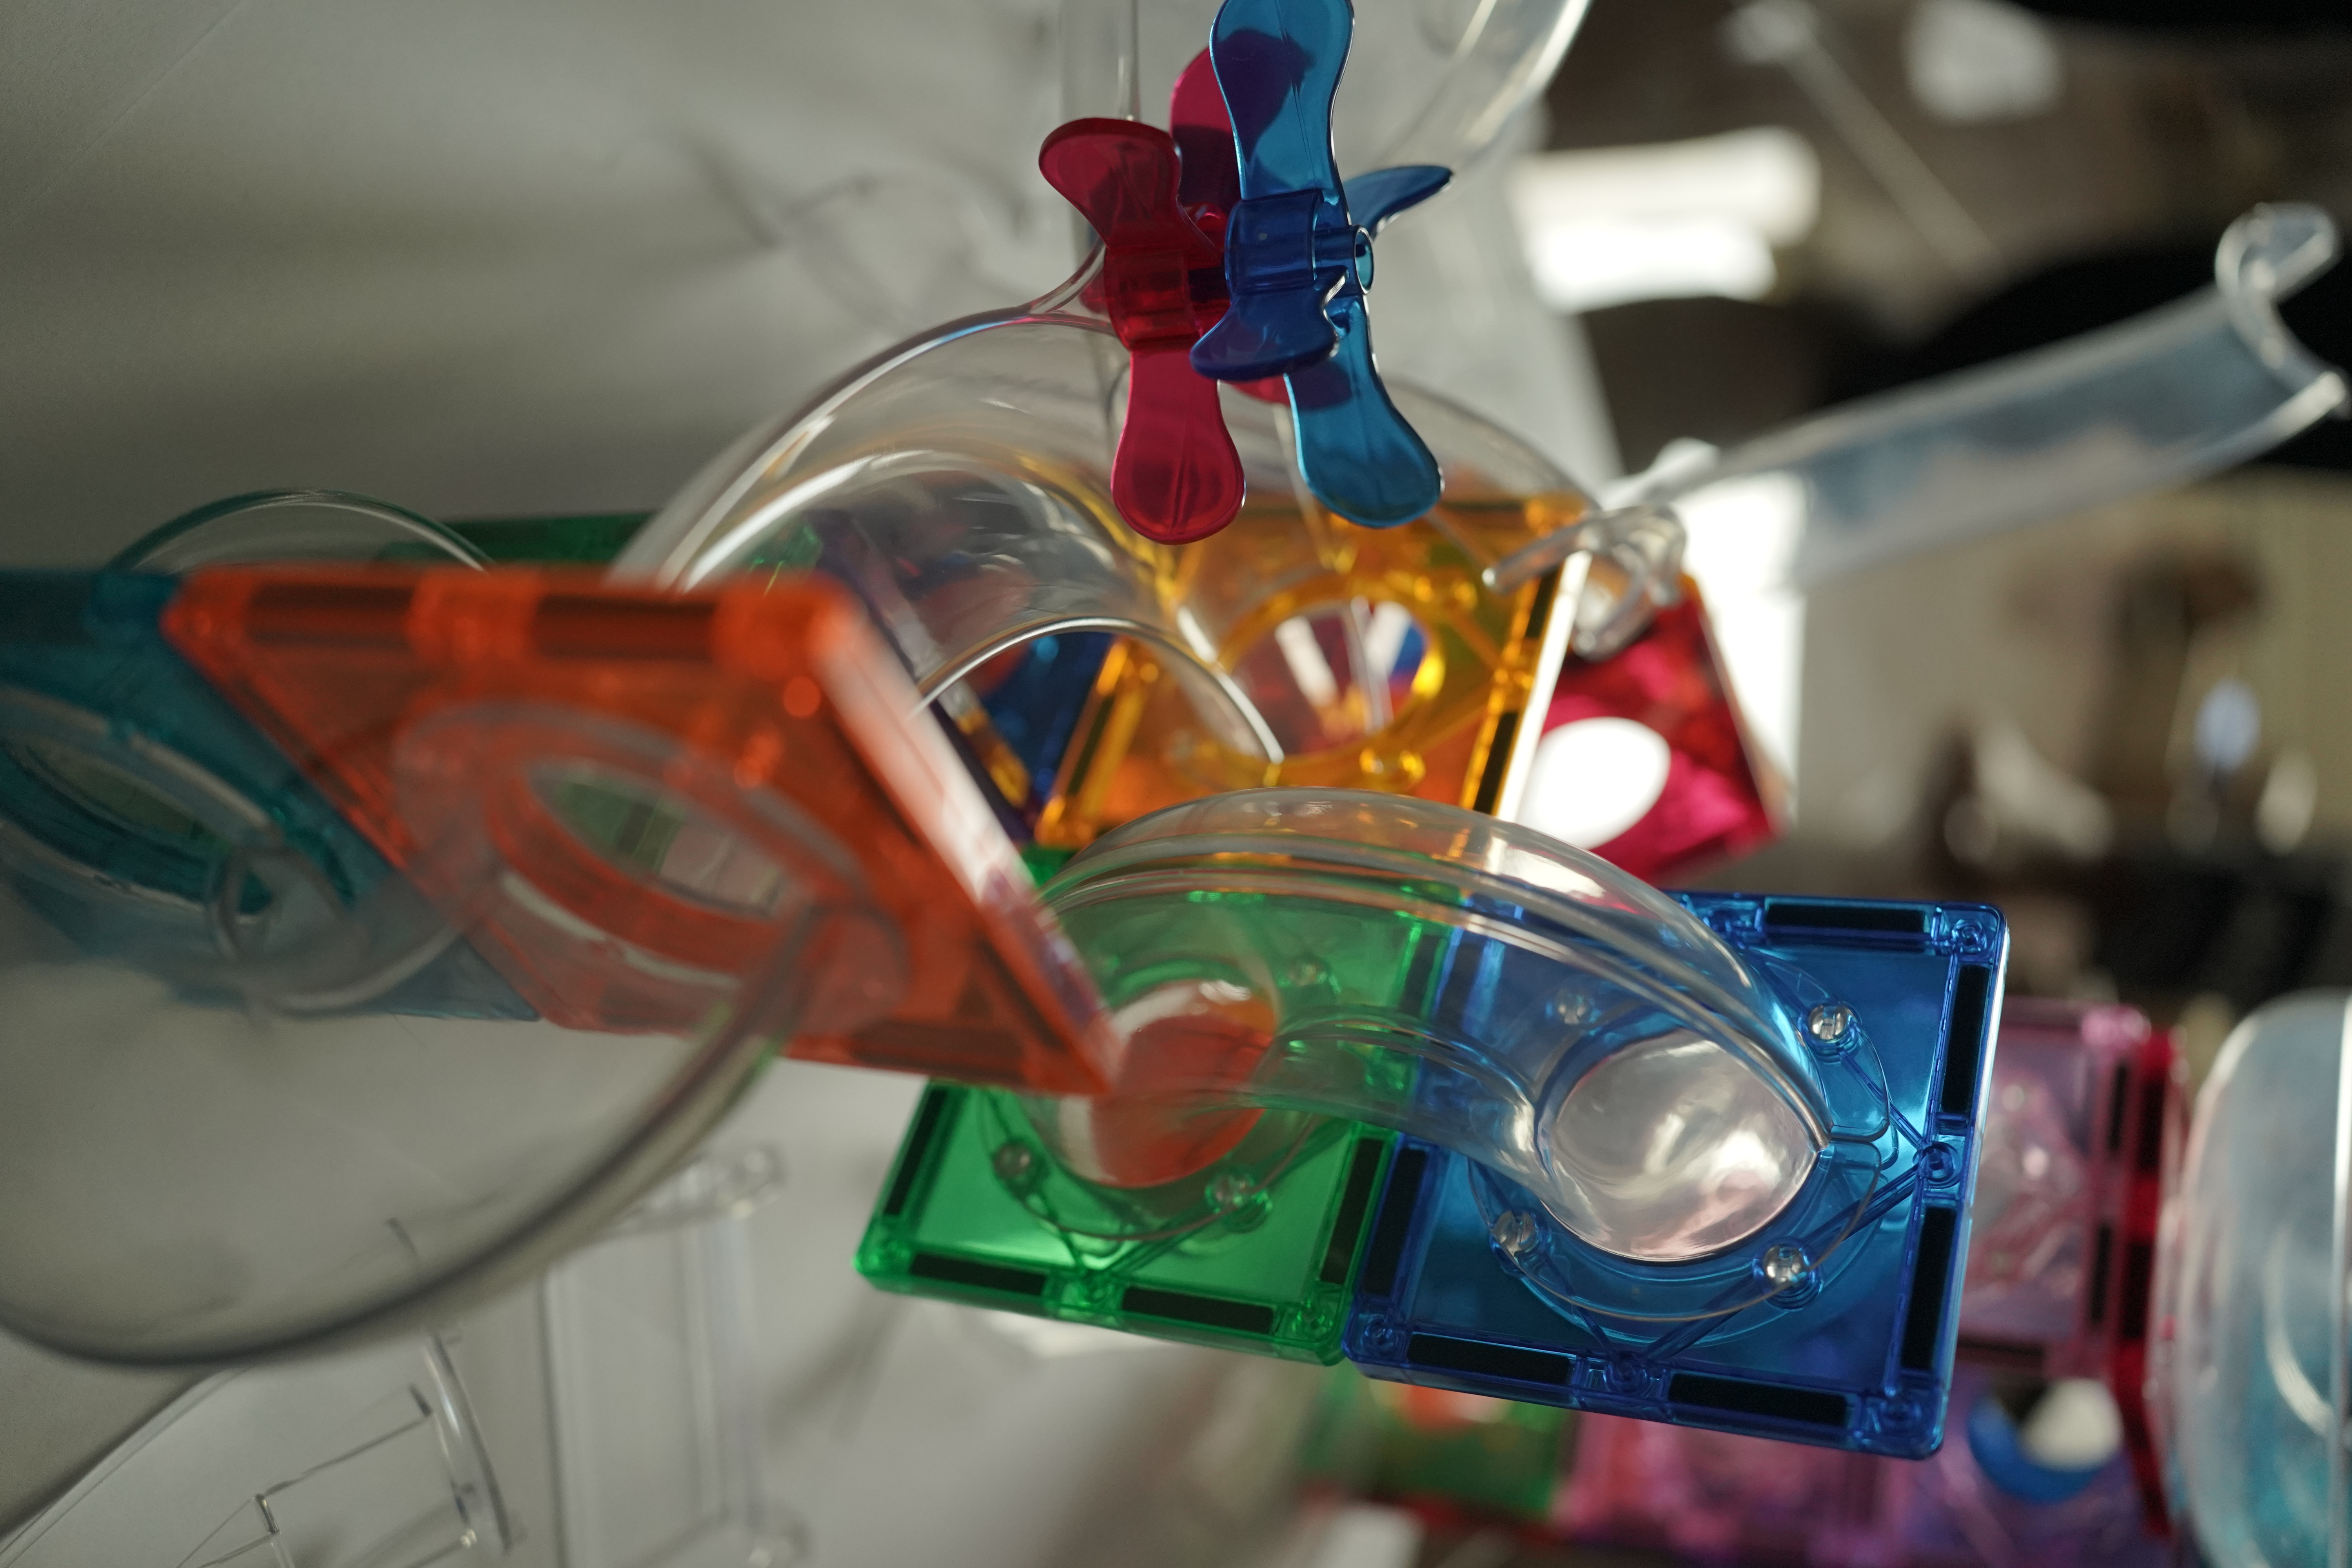
\includegraphics[angle=90,width=.5\linewidth]{Photos/Additional1.jpg}
  							\caption{Main Conveyer.}
  							\label{fig:sfig2}
						\end{subfigure}
						%%%%%%%%%%%%%%%%
						\begin{subfigure}{.5\textwidth}
						\centering
 							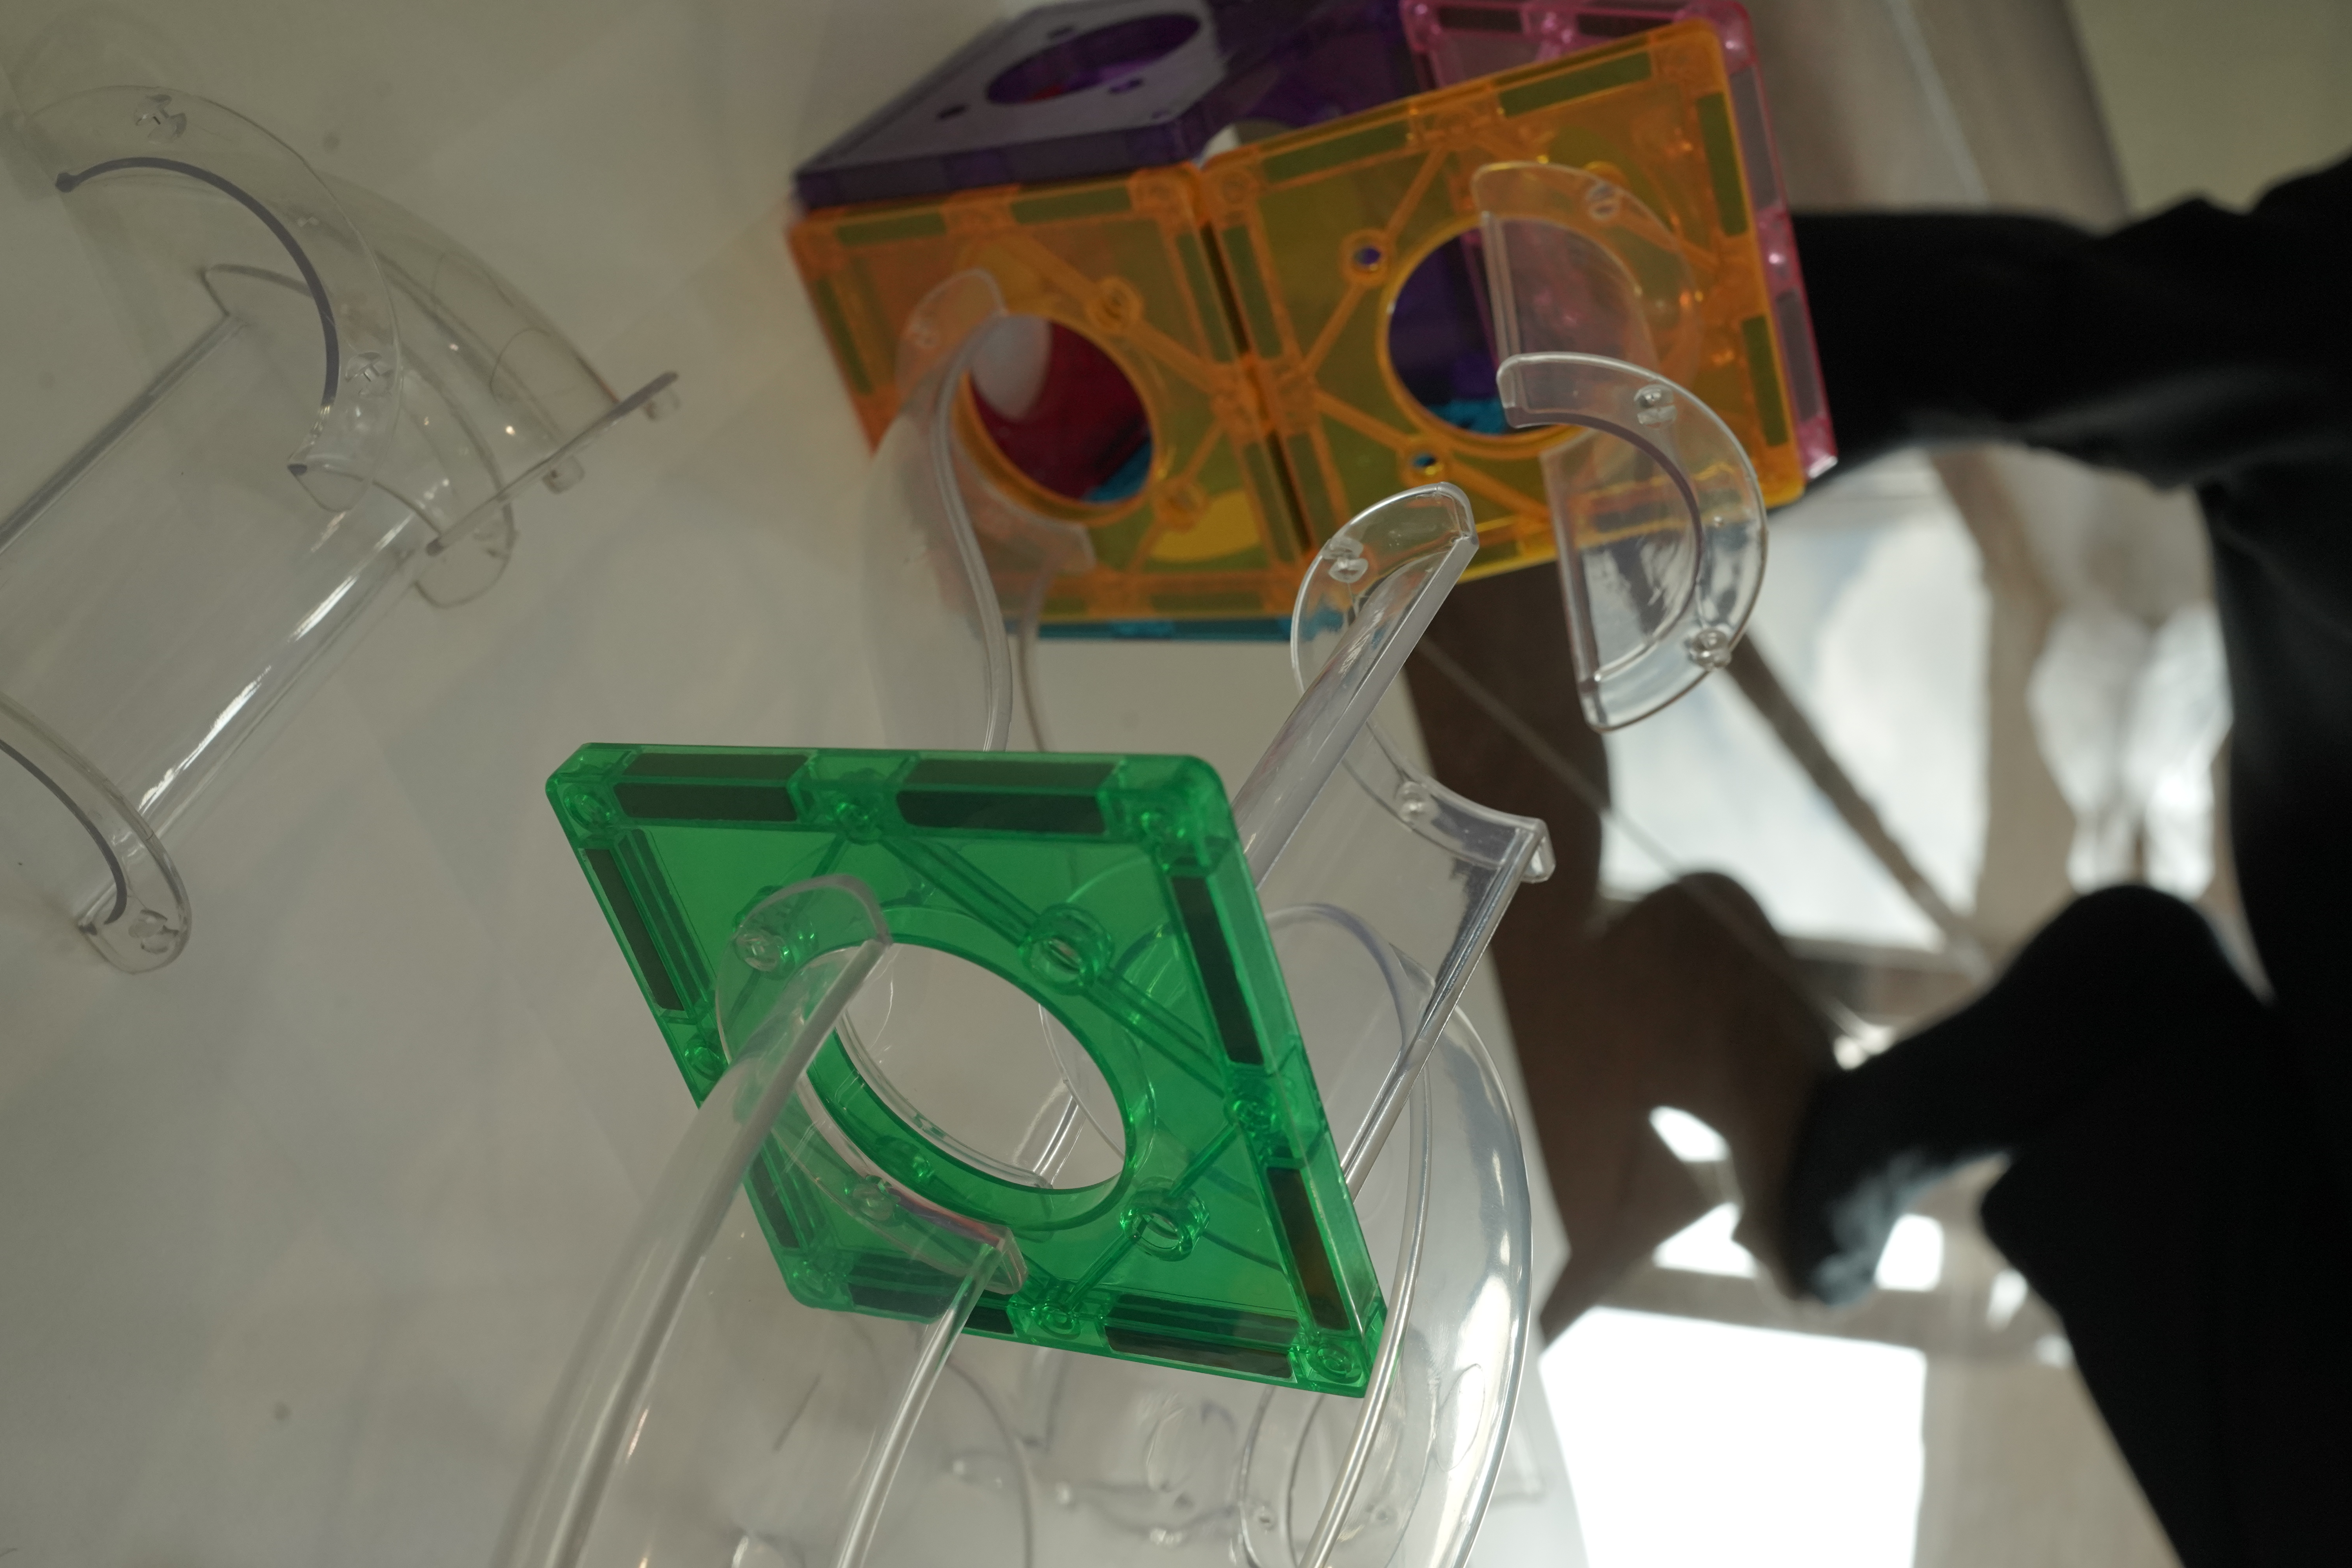
\includegraphics[angle=90,width=.5\linewidth]{Photos/In_Home.jpg}
  							\caption{House Drop Off Point.}
  							\label{fig:sfig3}
						\end{subfigure}
						%%%%%%%%%%%%%%%%%
						\begin{subfigure}{.5\textwidth}
						\centering
 							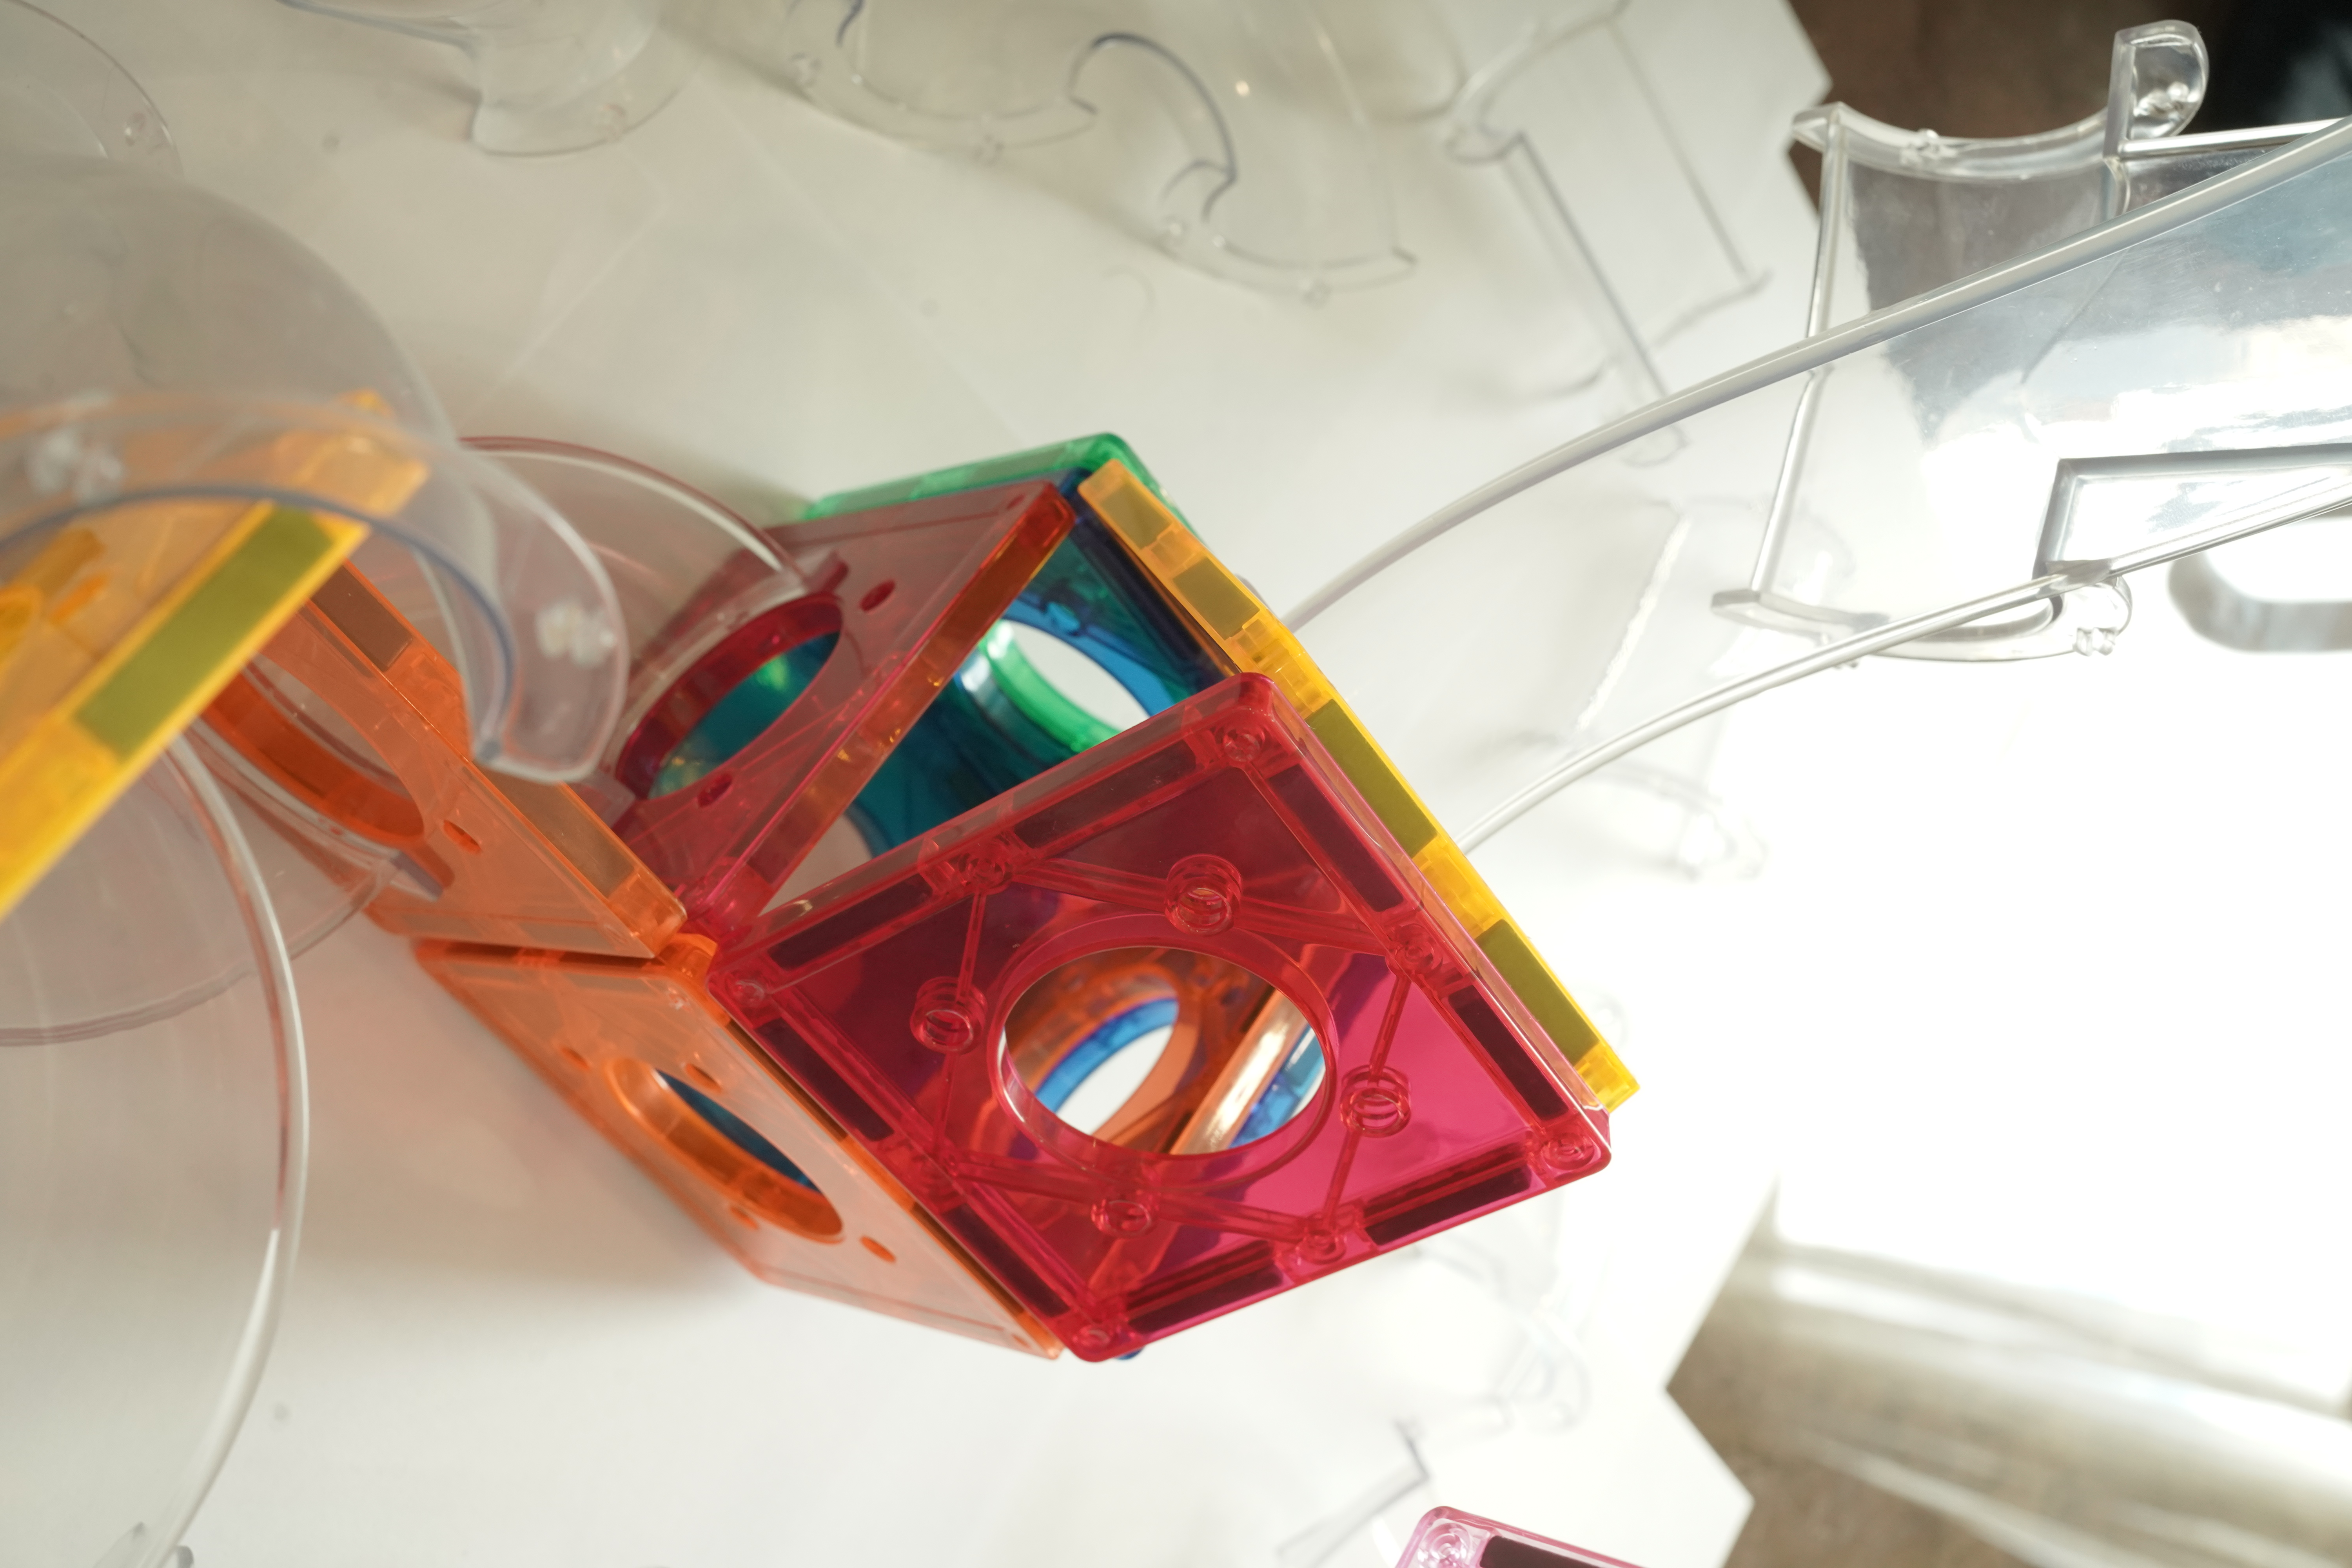
\includegraphics[angle=90,width=.5\linewidth]{Photos/residence_JOHN.jpg}
  							\caption{Residences of the base.}
  							\label{fig:sfig4}
						\end{subfigure}
					\caption{Components of The \textit{Suishan} Base.}
					\label{fig:fig}
				\end{figure}
				The design is a slider that can be used to transport both supplies and rebels. Many rebels use the slider to transport to another section of the basement. The main section is the one linked to the house which is the main entrance and exit that is used to gather the supply from the outside and swoop back in the slider. The fan is a path changer for any rebel that crosses the 3 ways or 2 ways slider.
				
				
			\subsection{Ethical questions or trade-offs the design raises.}
				With this design, \textit{Suishan} can’t accommodate many more survivors, which means that sometimes \textit{Suishan} can’t help those who aren’t rebels because of the low space and maze design of \textit{Suishan}. The trade-off is that \textit{Suishan} becomes very vulnerable against missiles or any artillery if the barrier is down. 
				
				
			\subsection{Reflect briefly (in writing) on how design can both oppress or empower in times of crisis.}
				This base can empower rebels against \textit{OJAAs}. With their base and symbol, they give humanity hope, allowing many people who are forsaken to get the morale boost in this time of crisis. Moreover, it serves as the main center for gathering scientists, soldiers, and doctors, which means it has enough accommodation in the darkest hour. Furthermore, with the strong mother base, humanity can conquer back any locations that \textit{OJAAs} has taken and bring more people to join the rebellion. 

		\end{document}
